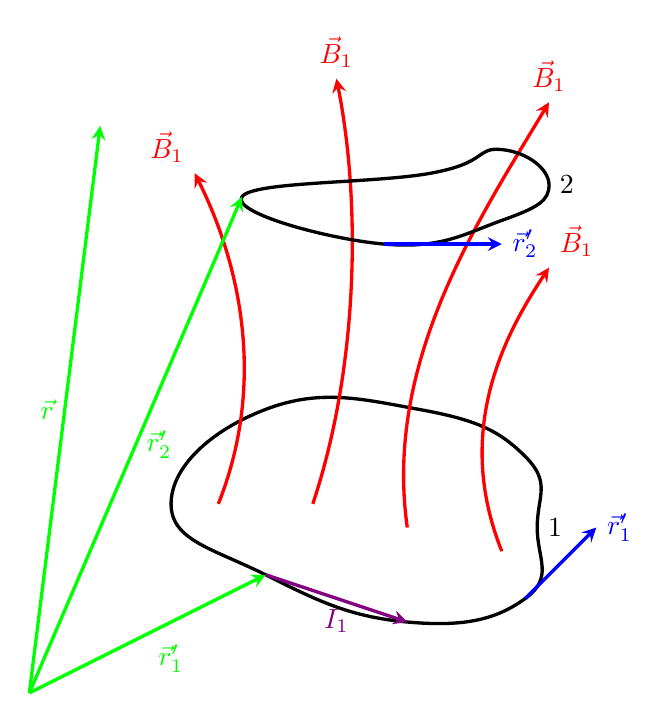
\begin{tikzpicture}[line width = 1.2pt, line join=round,x=1cm,y=1cm,>=stealth, scale = 3]
	% Schleife 1
	\coordinate (a) at (1,0.5);
	\coordinate (b) at (1.6,0.3);
	\coordinate (c) at (2.1,0.4);
	\draw plot [smooth cycle, tension=0.8] coordinates {(2.1,1) (1.65,1.2) (1,1.2) (0.6,0.8) (a) (b) (c) (2.15,0.7)} node [anchor=west] {$ 1 $};
	% Strom 1
	\draw [->, color=violet] (a) -- (b) node [anchor = north,midway] {$  I_1 $};
	% differentieller Weg 1
	\draw [->, color = blue]  (c) -- ++(0.3,0.3) node[anchor=west] { $ \dd  \vec{r}'_1 $ };
	% magnetische Flussdichte
	\draw [->,color=red] (0.8,0.8) .. controls (1,1.3) and (0.9,1.8) .. (0.7,2.2) node[anchor=south east]{$ \vec{B} _1 $};
	\draw [->,color=red] (1.2,0.8) .. controls (1.4,1.4) and (1.4,2.1) .. (1.3,2.6) node[anchor=south]{$ \vec{B} _1 $};
	\draw [->,color=red] (1.6,0.7) .. controls (1.5,1.4) and (1.9,2) .. (2.2,2.5) node[anchor=south]{$ \vec{B} _1 $};
	\draw [->,color=red] (2,0.6) .. controls (1.8,1.1) and (2,1.5) .. (2.2,1.8) node[anchor=south west]{$ \vec{B} _1 $};
	% Schleife 2
	\coordinate (ab) at (1.5,1.9);
	\coordinate (bb) at (0.9,2.1);
	\draw plot [smooth cycle, tension=0.8] coordinates {(2,2.3) (1.7,2.2) (bb) (ab) (2,2) (2.2,2.15) } node[anchor=west]{$ 2 $};
	% differentieller Weg 2
	\draw [->,color=blue] (ab) -- ++(0.5,0) node[anchor = west] { $ \dd  \vec{r}'_2 $ };
	% Ortsvektoren
	\draw [->,color=green] (0,0) -- (a) node[anchor=north west,midway] {$ \vec{r}' _1 $};
	\draw [->,color=green] (0,0) -- (bb) node[anchor=west,midway] {$ \vec{r}' _2 $};
	\draw [->,color=green] (0,0) -- (0.3,2.4) node[anchor=east,midway] {$ \vec{r}  $};
\end{tikzpicture}